\section{Disguise Execution Algorithm}

\begin{figure*}[ht!]
    \centering
    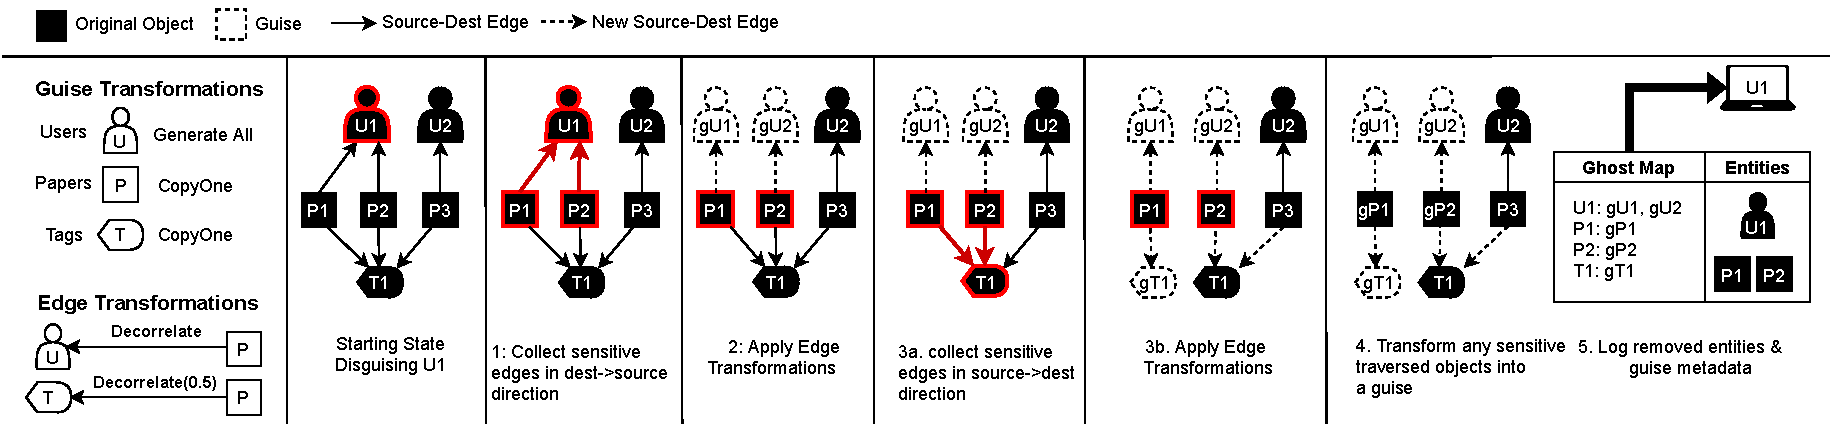
\includegraphics[width=\textwidth]{img/algo}

    \caption{Stages of \sys's execution when disguising user U1. Entities and edges detected as
    sensitive are outlined in red. Only the part of the entity graph relevant to unsubscription is shown.
    For simplicity, the specified guises policies apply for all attributes
    of the entity: a black ghost entity indicates that it is a full copy of the original.
    New edges indicates that the edge (foreign-key) value of the source has been changed to
    point to the specified dest.\\
    In this example, \sys decorrelates paper-tag edges only enough that the proportion of sensitive papers
    is at most the sensitivity threshold of 0.5, retaining one correlation between a sensitive
    paper P2 and the dest tag T1, and decorrelating the other sensitive paper P1 from the tag.}
    \label{fig:algo}
\end{figure*}


Given an application's schema and disguise spec, and an entity to be decorrelated as input,
\sys executes unsubscription as follows. Figure~\ref{fig:algo} illustrates each step.
\begin{enumerate}
    \item \textbf{Dest-Source Traversal:} \sys traverses the entity graph starting from the input entity,
        going down dest to source edges (and halting if it detects a cycle).
        \sys collects traversed edges as it traverses the graph.

    \item \textbf{Dest-Source Edge Policy Application:}
        Post-traversal, \sys acts on each collected edge instance according to the specified
        decorrelation relationship policy for that edge's type.

        \sys takes all edges of every unique dest entity, and applies policies as appropriate.
        Note that any sensitivity threshold less than $1$ requires that \emph{all} edges be decorrelated or
        deleted, depending on the developer's specified choice: all the sources of this dest are
        sensitive due to the nature of \sys's dest-source traversal.

        Any edges that should be deleted removes the source entity and any descendants.
        \sys generates new ghost dests using the real dest as template for any edges that should
        be decorrelated, and rewrites the source's edge attribute to be the ghost dest's
        identifier. If any edges are retained, \sys generates a ghost dest entity to replace the
        dest.

    \item \textbf{Source-Dest Edge Policy Application:}
        Next, \sys takes the sources of all traversed edge instances, and considers the set of
        edges from these sources to other dests \emph{not} traversed by \sys during the first
        traversal phase. In other words, these sources have multiple dests, at least one of which
        is transitively connected to the input entity.

        Intuitively, sources of edges traversed by \sys share a connection with the initial
        entity being decorrelated. Edges \emph{from} these sources to other dest entities may
        thus leak sensitive identifying information.

        \sys acts on these source-dest edges according to the specified edge policy for each edge's
        type. For each unique dest, \sys limits the proportion of edges of each type that connect
        to sensitive entities (the sources of traversed edge instances) to below the policy's
        sensitivity threshold by either decorrelating or deleting the sources.
        If \sys retains any edges from sensitive sources to the real dest, then \sys generates a
        ghost dest entity to replace the dest.

        Note that unlike the previous steps, this step considers edges from dests that may have
        many non-sensitive sources (\eg a particular tag may correlate with many stories by various
        authors).  \sys therefore may retain edges to sensitive sources when given a sensitivity
        threshold less than 1 and greater than 0, unlike in the previous step.

        \sys optionally allows developers to specify that edges have weaker or stronger edge
        policies in the source-to-dest direction than in the  dest-to-source direction. Weaker
        policies---higher sensitivity thresholds---allow \sys to retain links if \emph{only the
        source} is sensitive, but decorrelate or remove the link if \emph{both} the source and dest
        are sensitive. For example, perhaps a user wants to ensure that they are decorrelated from
        their reviews, but correlations between the review and the the paper authors can still be
        retained.

        Stronger policies may specify that the dest connected to sensitive sources should
        decorrelate \emph{all} correlations to the paper even from non-sensitive correlations.
        Developers specify such a policy with a sensitive threshold of -1. For
        example, perhaps the set of users with review conflicts to the paper can identify the
        author, even if the author is decorrelated from the paper. We see an example of this in
        Section~\ref{sec:hotcrp_example} (Figure~\ref{fig:pcs}).

    \item \textbf{Anonymizing Leaf Sources:}
        If any sensitive sources that are leaves (have no sources) remain, \sys generates a ghost source entity to replace this leaf.

        In Figure~\ref{fig:algo}, step 4, P1 and P2 are both leaves. \sys generates ghosts for both
        these papers: since these papers have \texttt{CopyOne} guises policies, ghost papers gP1
        and gP2 are identical to P1 and P2, and retain the edge attributes linking them to their
        respective dest tags and users.

    \item \textbf{Returning User Data:} \sys collects all removed entities that have either been
        replaced by ghost entities, or deleted entirely from the graph. \sys also records all
        generated ghost entity identifiers, and which ghost entities replaced which real entity.
        \sys returns both the removed entity data and this ghost entity metadata to the user.
\end{enumerate}

Note that \sys must decide \emph{which} ghost copies the template entity's attributes when the
developer selects a \texttt{CopyOne} guises policy for one or more attributes. \sys always
associates the copied ghost with as many non-sensitive entities as possible. For example, as shown
in Figure~\ref{fig:algo} step 3b, if \sys decorrelates sensitive papers from a dest tag with a
\texttt{CopyOne} policy, \sys chooses the ghost tag that remains associated with non-sensitive
papers to be the copy. This decision ensures that any unsensitive application
data remain as unaffected as possible when disguising another entity.
To optimize
\texttt{CopyOne} policies, \sys can simply retain the original template entity instead of producing
a copied ghost.
